\chapter{Verification and Validation Plan}
The methods used to size the design, as well as the product itself need to be verified and validated. For the methods, this means testing of individual computations as well as assessing the convergence of the final results (verification, see \autoref{sec:Method Verification}) and assessing the relevance of the method (validation, see \autoref{sec:Method Validation}). For the product, this means confirming it meets the requirements (verification, see \autoref{sec: Product verification}) and that it indeed can perform its envisioned mission (validation, see \autoref{sec: Product validation}).

\section{Verification}
\label{sec:Method Verification}

The designs are sized using iterative code. The code executes several independent analyses in a loop. After each analysis, parts of a global single source of truth object representing the aircraft are updated.

This setup allows to verify the particular analyses themselves. Per-analysis verification is described in the relevant sections of \autoref{ch:engineering_design}.

It is also necessary to ensure the iterative sizing converges. This is done by tracking the history of aircraft MTOM for each iteration step for each configuration. The results of the convergence study are shown in \autoref{fig:midtermIteration}. For the sizing of the final design, a similar convergence study shall be conducted.

\begin{figure}[h]
    \centering
    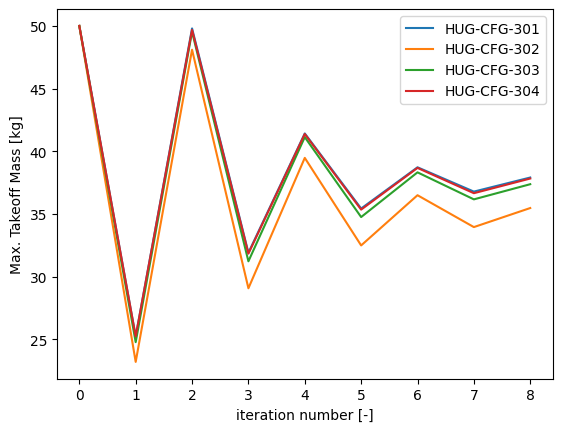
\includegraphics[width=0.6\linewidth]{figures/MidtermIteration.png}
    \caption{Convergence of maximu}
    \label{fig:placeholder}
\end{figure}

\section{Validation}
\label{sec:Method Validation}

The main goal for the methods for the Midterm Report is to provide numerical data for the trade-off. As such, a sensitivity study is conducted in \autoref{sec: sensitivity study} to assess whether the method predictions will not change to an extend that affects the trade-off with varying its assumptions.

For the Final Report, the goal of the method is to provide accurate numerical values used for subsystem design. As such, it can be verified by employing the same method to evaluate an existing aircraft, and compare the method's results with real aircraft data. This would require detailed information on the reference aircraft of choice. The method would also need to be general enough to accommodate both HUGO and the reference aircraft. The need for validation may thus be driving for the development of the Final Report methods.

% \section{Product verification}
% \label{sec: Product verification}

% Product verification concerns assuring that it meets the requirements. For the Midterm Report, this is mostly ensured by the sizing methods employed. That is, the aircraft design is updated after each analysis to meet the requirements (for example, wing loading, and thus wing area is adjusted after the matching diagram construction). For the Final Report, a compliance matrix addressing all the requirements shall be constructed and it shall be confirmed that the final design does satisfy every requirement.

% \section{Product validation}
% \label{sec: Product validation}
% The main purpose of HUGO is to allow for cheaper and more realistic high-speed tests of aeroservoelastic systems (HAR planforms in particular) than traditional wind tunnels. To specify whether the final product meets those goals, an aeroelastic analysis of the aircraft needs to be conducted and its costs need to be outlined and compared with existing aeroservoelastic testing methods.

% The aeroelastic analysis shall examine how the response of the wing differs between cantilever wing simulated in isolation and a model of the full aircraft. The cost analysis will be an iteration on the one from the Baseline Report \footref{url:baseline_report} updated with the properties of the final design.